\section{RAM}
\textbf{Random Access Memory (RAM)} is the internal memory of the digital system for storing data, program, and program result. It is a read/write memory which stores data until the machine is working. There are two types of RAM:

\begin{description}
    \item[Static RAM (SRAM)] which stores a bit of data using the state of a six transistor memory cell.
    \item[Dynamic RAM (DRAM)] which stores a bit data using a pair of transistor and capacitor which constitute a DRAM memory cell.
\end{description}

\subsection{SRAM}
Static random access memory (static RAM or SRAM) is a type of RAM that uses latching circuitry (flip-flop) to store each bit. \figref{SRAM} shows an SRAM cell.

\begin{figure}[H]
	\begin{center}
		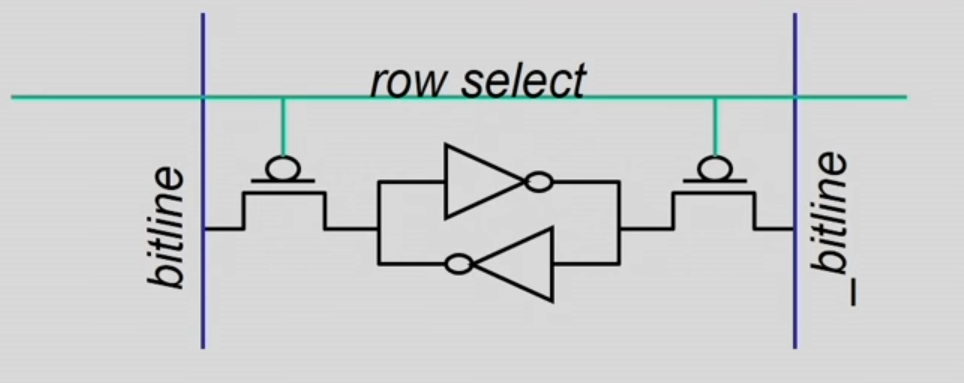
\includegraphics[width=5in]{images/SRAM.png}
		\caption{Static RAM cell}
		\label{SRAM}
	\end{center}
\end{figure}

SRAM cell can store 1 bit of information which consists of a row line and a bitline. A pair of bit lines is used for storage of every bit, one is bitline and the other one is bitline compliment. Bitline compliment is a logical compliment of the bitline. 

\par Two cross coupled NOT gates are connected by two transistor, which are connected to the row select. So, once a particular row is selected both T1 and T2 is going to be in on position. So, whatever value is there in the bitline it flows into the not gates. The value in the bitline will get stored inside the two cross coupled NOT gates loop.
Hence, transistor will basically act as a switch in this context.

\subsubsection{Large SRAM implementation}
These SRAM memory cells, consisting of six transistors, organized as rows and columns to get an organized structure for the main memory. Address needs to be generated consisting two components, \ie 'n' bits representing the rows and 'm' bits representing the columns. 

\par While reading from the memory, the row is chosen by using an n to \(2^(n)\) decoder.Once the row is selected, the entire contents of the row are transferred to a sense amplifier. And, the single bit extracted by selecting from 'm' column number.

\par Read sequence is as follows:
\begin{enumerate}
    \item Address decode
    \item Drive row select
    \item Selected bit-cells drive bitlines (entire row is read together)
    \item Column select (Data is ready)
\end{enumerate}

\subsection{DRAM}
Dynamic random access memory (Dynamic RAM or DRAM) is a type of random access memory that stores each bit of data in a memory cell, usually consisting of a tiny capacitor and a transistor, both typically based on metal-oxide-semiconductor (MOS) technology. 

\begin{figure}[H]
	\begin{center}
		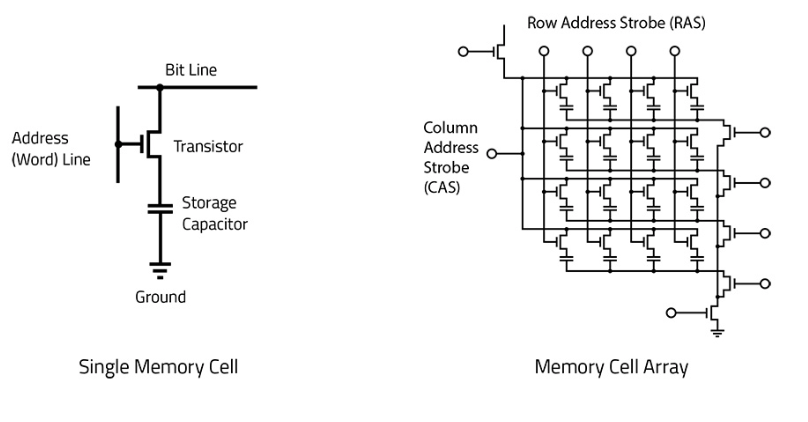
\includegraphics[width=5in]{images/DRAMCell.png}
		\caption{Dynamic RAM cell}
		\label{DRAMCell}
	\end{center}
\end{figure}

Bits are basically stored as charges on the capacitor and a memory cell lose charge when it is read. When there exists a potential difference between the parallel plates of a capacitor, it is called as logic 1. And, when the potential difference between the two parallel plates of a capacitor is less than a threshold value, then it is called as logic 0. 

\begin{itemize}
    \item Bits are stored as charges on capacitor.
    \item Memory cell loses charge when read.
    \item Memory cell loses charge over time.
    \item A flip flop in sense amplifier amplifies and regenerates the bitline and data bit is multiplexed out of it.
\end{itemize}

Since the capacitor discharges over time, the information stored eventually fades unless the capacitor is periodically REFRESHed. This is where the 'D' in DRAM comes from. It refers to Dynamic as opposed to static in SRAM.

\subsubsection{DRAM vs SRAM}
\textbf{DRAM}
\begin{itemize}
    \item Slower access (capacitor)
    \item Higher density (transistor, capacitor cell)
    \item Lower cost
    \item Requires refresh (power, performance, circuitry)
    \item Manufacturing requires putting capacitor and logic together
\end{itemize}

\clearpage
\textbf{SRAM}
\begin{itemize}
    \item Faster access (no capacitor)
    \item Lower density (6 transistor cell)
    \item Higher cost
    \item No need for refresh
    \item Manufacturing compatible with logic process (no capacitor)
\end{itemize}

\begin{highlight}
    Density plays a crucial role in accommodating larger memory in a smaller size memory. DRAM is preferred in order to implement the primary memory.
\end{highlight}

\subsubsection{Asynchronous \& Synchronous DRAM}
In different generations of dynamic RAM there is an improvement in the speed as well as the reduction in the power consumption. Asynchronous Dynamic RAM can be considered as the oldest generation of dynamic RAM. Asynchronous DRAM means that the RAM is not synchronized with the CPU clock. The obvious disadvantage of this particular type of RAM was that then CPU does not know the exact timing at which the data will be available from the RAM on the input output bus. 

\par This problem has been overcome by the next generation of RAM, which is known as the synchronous DRAM. In case of SDRAM, the RAM is synchronized with the CPU clock. Now, the advantage of this type of SDRAM is that the CPU or to be precise, the DRAM memory controller knows the exact timing or the number of cycles after which the data will be available on the bus. And hence, the CPU does not need to wait for the memory access. This also results in increasing memory read \& write speeds. The synchronous DRAM modules are operated at 3.3V. SDRAM or synchronous DRAM is also known as the Single Data Rate SDRAM as the data is transferred at the every rising edge of the clock cycle.

% \par There are a total two types of different frequencies associated with DRAM. The first is the input output clock frequency and the second is the RAM internal clock frequency. The input output clock frequency is the frequency at which the data is being transferred between the RAM and the memory controller. And, the internal clock frequency of the RAM is the frequency which is being used by the RAM for the internal operations. In case of synchronous DRAM, input output clock frequency and the internal clock frequency of the RAM are same. For \eg suppose if the internal clock frequency of the RAM is 100 MHz then, the input output clock frequency is also 100 MHz. Suppose if you find the PC-100 specification on the SDRAM module, it means that the input output clock frequency is 100 MHz and the data that is being transferred between this RAM and the memory controller is at the rate of 100 mega transfers per second and if the data bus is 64 bit wide, then the data rate in terms of the bits per second will be 100 MHz into 64 bits. Which is 800 Megabytes per second.

\subsubsection{Interleaving}
One of the main issues in accessing a single monolithic memory is that A single monolithic memory array takes long to access and does not enable multiple accesses in parallel.

\par The solution to this problem is to divide the entire memory into multiple banks that can be accessed independently (in the same cycle or in consecutive cycles).

\par The key design issue is to map the data into different banks. This issue is resolved by the process referred to as Interleaving, or Banking. In interleaving, 
\begin{itemize}
    \item Address space partitioned into separate banks
    \item No increase in data store area
    \item Bits in address determines which bank an address maps to
    \item Cannot satisfy multiple accesses to the same bank
    \item Crossbar interconnect in input as well as output
    \item Bank conflicts: Two accesses to the same bank are difficult to handle
\end{itemize}

One simple way of implementing banking is odd even separation. All the even addresses can be considered as mapped to bank 0 and all the odd addresses can be considered as mapped to bank 1.

\par The address provided to read the data is typically referred as "logical address". Logical address is translated to a physical address before it is presented to the DRAM. The physical address is made up of the following fields:
\begin{itemize}
	\item Bank Group
	\item Bank
	\item Row
	\item Column
\end{itemize} 

These individual fields are then used to identify the exact location in the memory to read-from or write-to. 

\subsubsection{Organization of the DRAM}
DRAM consists of multiple hierarchies of channels, DIMM(Dual Inline Memory Module), rank, chip, bank, row columns, and B-cells/ Memory Cells. A digital system can request data reads from memory at any point of time. To read from the memory, address has to be provided and to write to the memory, data \& address has to be provided. 

\figref{DRAMOrganization} shows the organization of the DRAM.

\begin{itemize}
    \item The processor may have multiple channels \ie it may have multiple address buses or data buses. 
    \item A channel is formed by joining multiple DIMMs.
    \item The DIMM has a front side (known as rank 0) and a back side (known as rank 1).
    \item Rank is a set of chips that respond to the same command and same address at the same time, but with different pieces of requested data. 
    \item Both ranks are usually provided with a common address, and one rank, either rank 0 or rank 1, gives the corresponding data.
    \item Rank comprises of multiple chips.
    \item Each chip holds and shares a sub component of the entire data held by a rank.
    \item Each chip has a 3D structure consisting multiple banks with each bank consisting a layer of rows and columns. 
    \item Breaking down a bank, each bank consists of rows as well as columns.
\end{itemize}

\begin{figure}[H]
	\begin{center}
		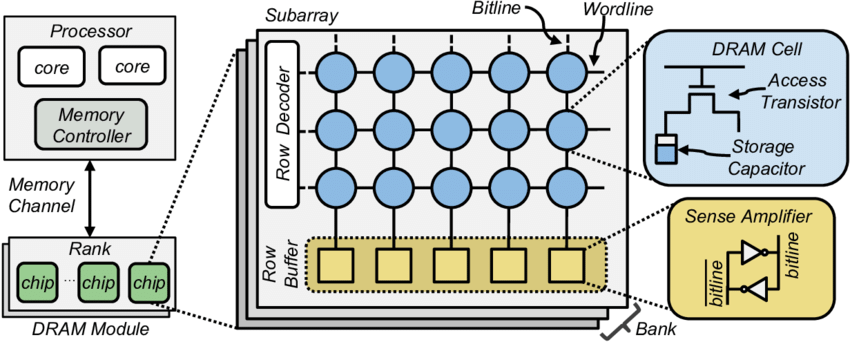
\includegraphics[width=\textwidth]{images/DRAMOrganization.png}
		\caption{Organization of the DRAM}
		\label{DRAMOrganization}
	\end{center}
\end{figure}

Going down another level, DRAM consists of a page mode structure. DRAM bank is a 2D array of cells which consists of rows and columns. Each Bank contains the following:

\begin{itemize}
	\item Memory Arrays
	\item Row Decoder
	\item Column Decoder
	\item Sense Amplifiers
\end{itemize} 

Once the Bank Group and Bank have been identified, the Row part of the address activates a line in the memory array. This is called the "Word Line" and activating it reads data from the memory array into "Sense Amplifiers". Sense amplifier are kept in row buffers. The Column address then reads out a part of the word that was loaded into the Sense Amplifiers. The width of the column is called the "Bit Line".

\par The width of a column is standard it is either 4 bits, 8 bits or 16 bits wide and DRAMs are classified as x4, x8 or x16 based on this column width. Another thing to note is that, the width of the data bus is same as the column width.

\clearpage

\subsubsection{DRAM Subsystem}
The DRAM talks to the ASIC or FPGA through the system called as the DRAM Subsystem. DRAM Subsystem is made up of 3 components:

\begin{itemize}
	\item The DRAM memory
	\item A DRAM PHY
	\item A DRAM Controller	
\end{itemize} 

\begin{figure}[H]
	\begin{center}
        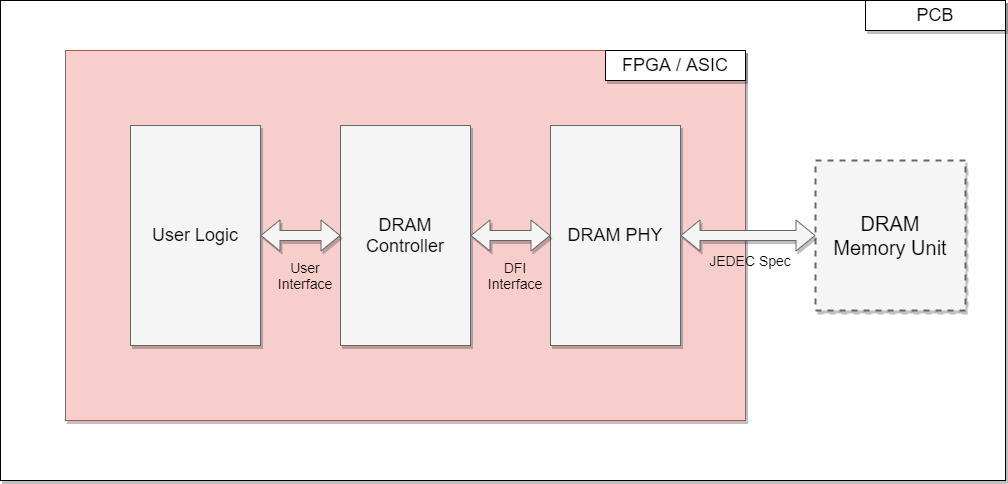
\includegraphics[width=\textwidth]{images/DRAMSubsystem.png}
		\caption{DRAM Subsystem}
		\label{DRAMSubsystem}
	\end{center}
\end{figure}


\begin{table}[H]
    \centering
    \begin{tabular}{||p{0.25\linewidth} ||  p{0.7\linewidth}||}
    \hline
    % \begin{tabular}{ll}
    \textbf{Block} & \textbf{Description} \\ [0.5ex] \hline  \hline 
    Physical (PHY) Layer     &   The direct interface to the external DRAM memory bus. Instantiates logic resources to generate the memory clock, control/address signals, and data/data strobes to/from the memory. Executes the DRAM power-up and initialization sequence after system reset. Performs read data capture timing training calibration after system reset, and adjusts read data timing using (IDELAY) elements.\\ \hline
    
    Controller     &  Generates memory commands (\eg Read, Write, Precharge, Refresh) based on commands from the User Interface block. Optionally, can implement a bank management scheme to reduce overhead with opening and closing of bank/rows. The controller logic takes over the DRAM address/control bus after successful completion of DRAM memory initialization and read timing calibration by the PHY layer.\\ \hline
    
    User Interface     & Custom interface for the user specific application to issue commands and write data to the DRAM memory interface, and to receive read data from the DRAM memory interface.\\ \hline
    
    Clocking / Reset Logic  & Generates clocks using Digital Clock Manager (DCM) module. Synchronizes resets to the various clock domains used in rest of design.\\ \hline    
    \end{tabular}
    \caption{DRAM Memory Interface Design Major components \& Descriptions}
    \label{tab:DRAMComponents}
\end{table}

\clearpage

The DRAM is soldered down on the board. The PHY and controller, along with user logic are typically part of the same FPGA or ASIC. The interface between the user logic and the controller can be user defined and need not be standard. When the user logic makes a read or write request to the controller, it issues a logical address. The controller then converts this logical address to a physical address and issues a command to the PHY. The Controller and PHY talk to each other over a standard interface called the DFI interface. The PHY then does all the lower level signaling and drives the physical interface to the DRAM. This interface between the PHY and memory is specified in the JEDEC standard. Think of the controller as the brains and the PHY as the brains.

\par When you activate a row, the whole page is loaded into the Sense Amplifiers, so multiple reads to an already open page are lesser expensive because you can skip the first step of row activation. The controller typically has the capability to re-order requests issued by the user to take advantage of this. To do the re-ordering it uses a small cache or TCAM and always returns the latest data, so you don't have to worry about stale data or collisions occurring because of this re-ordering done by the controller. The PHY contains the analog drivers and provides the capability to tweak registers to increase drive strength or change terminations, in order to improve signal integrity.



\subsubsection{Basic DRAM Controller Operation}

\textbf{DRAM Commands Issued by the Controller:} The commands are detected by the memory using these control signals: Row Address Select (RAS), Column Address Select (CAS), and Write Enable (WE) signals. Clock Enable (CKE) is held High after device configuration, and Chip Select (CS) is held Low throughout device operation.

\textbf{DRAM Memory Commands:}
\begin{description}
    \item [Precharge Command] It is used to deactivate the open row in a particular bank. The bank is available for a subsequent row activation a specified time (tRP) after the Precharge command is issued. 
    \item Precharge command:
    \begin{enumerate}
        \item Destructive read: Any read operation that is carried out on a capacitor, will discharge the charges that exist over the capacitor plates leading to a 0 potential layer \ie any reading operation will delete the value stored.
        \item The existing value in the row buffer should be stored back for a new read command.
        \item The operation of storing the contents in the row buffer back to the appropriate row is known as Precharge.
    \end{enumerate}

    \item [Auto Refresh Command] DRAM devices need to be refreshed regularly after a certain time period. The circuit to flag the Auto Refresh commands is built into the controller. The controller issues an Auto Refresh command after it has completed its current burst. Auto Refresh commands are given the highest priority in the design of the controller. 

    \item [Active Command] Before any read or write commands can be issued to a bank within the DRAM memory, a row in the bank must be activated using an active command. After a row is opened, read or write commands can be issued to the row.

    \item [Read Command] The Read command is used to initiate a burst read access to an active row. The values in registers select the bank address \& the starting column location in the active row. After the read burst is over, the row is still available for subsequent access until it is precharged. 

    \item [Write Command] The Write command is used to initiate a burst write access to an active row. The values in registers select the bank address \& the starting column location in the active row. DRAMs use a Write Latency (WL) equal to Read Latency (RL) minus one clock cycle. \\
    \( Write Latency = Read Latency - 1 = (Additive Latency + CAS Latency) - 1 \)    
\end{description}

DRAM Controller Operation is as follows:

\begin{itemize}
    \item In order to carry out the instruction execution with the help of an instruction pipeline, during the fetch stage cache memory will be used. If the required instruction or data is not available even in the last level cache then DRAM is required.
    \item Main processing unit has to communicate with the physical DRAM device and that communication is carried out by the DRAM controller. The controller itself has it's own latency called as Controller latency.
    \item Multiple requests coming from multiple tiles or multiple processors queue up inside the DRAM controller. These requests have to be scheduled in order to be executed by the DRAM controller resulting in Queuing delay \& scheduling delay. 
    \item Once scheduling is done, these requests have to be converted into a couple of basic commands.
    \item Appropriate commands are then propagated from the controller to the physical memory and generating bus latency. 
    \item Once the request reaches the physical memory unit, it has to split into column address and row address.
    \item There are different scenarios while handling a request:
    \begin{itemize}
        \item Opened Row Scenario: A scenario where a given row is already kept in the row buffer is known as a open row scenario. In this scenario, only a Column Address Strobe (CAS) is required. There is no need of Activate command.
        \item Closed Row Scenario: A scenario where a given row is not already kept in the row buffer is known as a closed row scenario. Access to a closed row is as follows:
        \begin{itemize}
            \item Activate command
            \item Read/Write command 
            \item Precharge command closes the row and prepares the bank for next access
        \end{itemize}
        \item Row conflict Scenario: In this scenario, some other row is already open. In this case row has to be closed first and then Row Address Strobe (RAS) and Column Address Strobe (CAS) has to be given one after another with appropriate timing gap between them.
    \end{itemize}
    \item The physical memory unit returns the data back to the controller generating bus latency.
    \item Once data reaches DRAM controller, the controller transfers it to the CPU or the last level cache.
\end{itemize}



\subsubsection{Internal Physical Structure of DRAM}

\begin{figure}[H]
	\begin{center}
		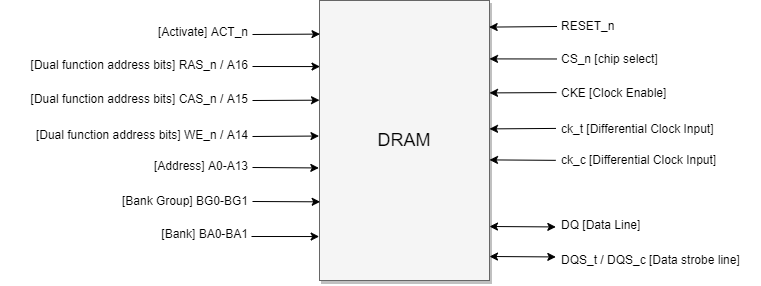
\includegraphics[width=\textwidth]{images/DRAMPHY.png}
		\caption{Top Level DRAM block diagram}
		\label{Top Level}
	\end{center}
\end{figure}

Usually, DRAM has clock, reset, chip-select, address and data inputs as shown in \figref{Top Level}. The \figref{DRAM ports} mentions all the pins in detail.

\begin{figure}[H]
	\begin{center}
		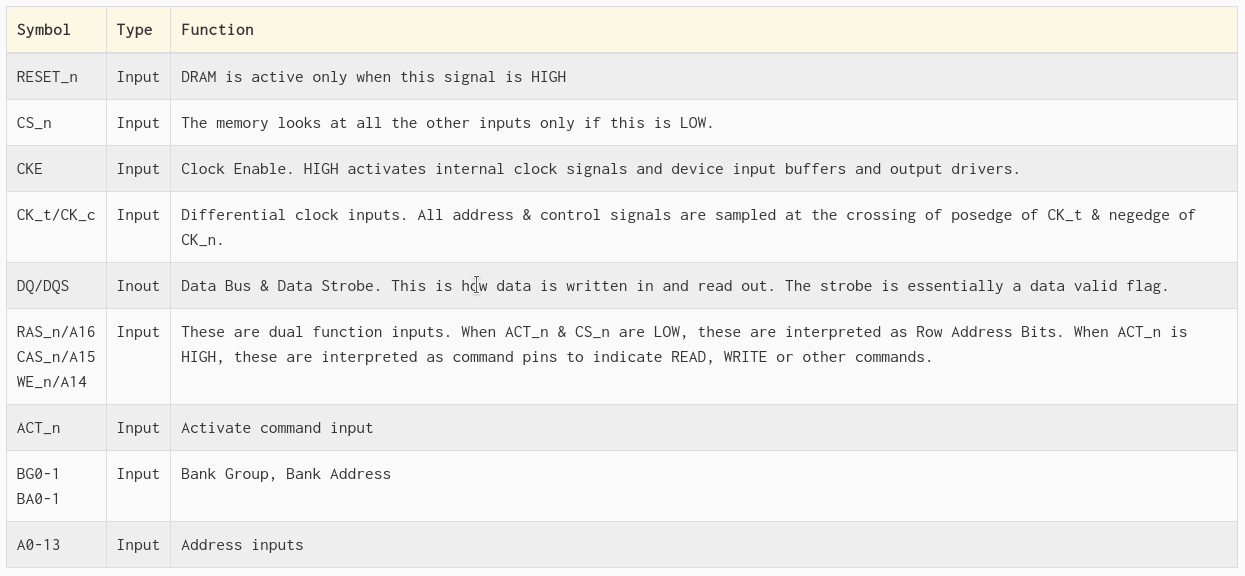
\includegraphics[width=\textwidth]{images/DRAMPorts.png}
		\caption{DRAM block diagram}
		\label{DRAM ports}
	\end{center}
\end{figure}